% =========================================================================
% Veritas: Version-Aware Enterprise Policy Intelligence
% IEEE Journal Manuscript — Camera-Ready
% Author: Suyash Pradhan
% All numbers verified against actual result files in results/ directory.
% Commit: 61d64b71c298c3c505f2eeeef3c94829dfb55f75
% =========================================================================
\documentclass[journal]{IEEEtran}

\usepackage{cite}
\usepackage{amsmath,amssymb,amsfonts}
\usepackage{algorithm}
\usepackage{algorithmic}
\usepackage{graphicx}
\usepackage{booktabs}
\usepackage{multirow}
\usepackage{array}
\usepackage{tabularx}
\usepackage{url}
\usepackage{microtype}
\usepackage{textcomp}
\usepackage{balance}

% ----- Macros -----
\newcommand{\sys}{Veritas}
\newcommand{\ms}{\,\mathrm{ms}}
\newcolumntype{Y}{>{\centering\arraybackslash}X}
\newcolumntype{Z}{>{\raggedright\arraybackslash}X}
\newcommand{\D}{\mathbb{D}}

\setlength{\textfloatsep}{4pt plus 1pt minus 1pt}
\setlength{\floatsep}{4pt plus 1pt minus 1pt}
\setlength{\intextsep}{4pt plus 1pt minus 1pt}
\setlength{\dbltextfloatsep}{4pt plus 1pt minus 1pt}
\setlength{\dblfloatsep}{4pt plus 1pt minus 1pt}
\setlength{\abovecaptionskip}{2.5pt plus 1pt minus 1pt}
\setlength{\belowcaptionskip}{1.5pt plus 1pt minus 1pt}
\setlength{\abovedisplayskip}{3.5pt plus 1pt minus 1pt}
\setlength{\belowdisplayskip}{3.5pt plus 1pt minus 1pt}
\setlength{\abovedisplayshortskip}{2pt plus 1pt}
\setlength{\belowdisplayshortskip}{2pt plus 1pt}



\begin{document}

\title{\sys{}: Version-Aware Enterprise Policy Intelligence via
Incremental Knowledge Compilation and Adaptive Multi-Tier Retrieval}

\author{Suyash~Pradhan%
\thanks{S. Pradhan is with the Department of Computer Science and Engineering
(e-mail: suyashpradhan06@gmail.com).}}

\markboth{IEEE Journal Manuscript}{\sys{}: Version-Aware Enterprise Policy Intelligence}

\maketitle

% =========================================================================
\begin{abstract}
Enterprise policy repositories undergo continuous revision, requiring historical
and active provisions to coexist in queryable form under strict role-based access.
Conventional retrieval-augmented generation (RAG) models rank evidence primarily by
semantic similarity, incurring four operational risks: temporal version inversion,
full-corpus re-indexing overhead, generative latency on deterministic lookups, and
cross-scope authorization leakage. We present \sys{}, an enterprise policy intelligence
system that formulates retrieval as a constrained systems problem: a composite eligibility
predicate $E(c,u,t_q)=V(c,t_q)\cdot A(c,u)$ enforces date-bounded validity and role authorization
prior to evidence admission and reranking. \sys{} integrates this with a seven-stage SHA-256
incremental compiler, an adaptive four-tier query router, and a calibrated NLI verification layer.
Across a 21-policy, 128-chunk enterprise corpus evaluated on a 301-query benchmark, \sys{} achieves
100.0\% authorization/scope decision correctness (versus 46.84\% for an unrestricted baseline) and 82.72\% overall
version resolution rate (86.30\% local and 89.53\% cloud version-selection accuracy on answered queries). While
free-text exact-match correctness is 27.91\% (token F1: 0.3516), which may be partly attributable to 4-bit local quantization, high citation
precision (0.7973) indicates that most emitted citations correspond to authoritative evidence (with citation recall of 0.2487
reflecting section-level chunk granularity) and adversarial refusal accuracy (88.89\% local, 100.0\% cloud)
provides evidence of compliance-boundary enforcement. The incremental compiler delivers $5{,}059.72\times$ speedup on hash
no-op updates and $488.75\times$--$494.19\times$ on sparse chunk mutations ($O(|\Delta|\cdot d)$ dominant
embedding complexity). Isotonic calibration reduces calibration-split ECE from 0.5840 to 0.000 (Brier
score: 0.5855 to 0.1839), while runtime ECE rises to 0.2954 under heterogeneous query distributions,
revealing distribution sensitivity. Deterministic routes resolve 54.15\% of queries at P50 $< 24\,\mathrm{ms}$,
yielding an end-to-end median latency of $29.65\,\mathrm{ms}$.
\end{abstract}


\begin{IEEEkeywords}
Retrieval-augmented generation, temporal information retrieval, version-aware
retrieval, incremental indexing, enterprise knowledge management, adaptive query
routing, confidence calibration, natural language inference.
\end{IEEEkeywords}

% =========================================================================
\section{Introduction}
\IEEEPARstart{E}{nterprise} governance, corporate administration, information
security, and regulatory compliance depend on policy documents that are revised
continuously. Corporate travel allowances, parental leave provisions, remote-work
rules, and security controls each undergo periodic amendment, requiring retrieval
mechanisms that can distinguish historical validity from current applicability
while respecting authorization boundaries.

Conventional retrieval-augmented generation (RAG) architectures primarily rank
semantic similarity over document collections \cite{lewis2020rag,gao2024rag_survey}.
Within enterprise policy repositories, four operational risks are particularly
important. \textbf{(1) Temporal version inversion:} semantically similar but
superseded clauses are retrieved for current queries, or obsolete provisions are
returned for historical inquiries \cite{campos2014temporal,huwiler2025versionrag,timelyrag2026}.
\textbf{(2) Re-indexing overhead:} small document changes trigger
corpus-wide re-embedding. \textbf{(3) Generative latency:} deterministic
policy facts incur avoidable autoregressive inference. \textbf{(4) Scope
leakage:} retrieval over unpartitioned repositories exposes departmental or
confidential information to unauthorized users
\cite{almasoud2026sdrag,mu2026securerag}.

This paper investigates the following central research question: \textit{Can an
enterprise policy retrieval architecture simultaneously enforce date-bounded
temporal validity and role-based authorization constraints while reducing
unnecessary generation latency and incremental compilation overhead, without
degrading retrieval accuracy on legitimate requests?}

To answer this question, \sys{} treats policy retrieval not merely as a vector
similarity search, but as a constrained systems problem. While individual components
such as dense embeddings, lexical indexes, cross-encoders, and NLI classifiers exist
in isolation, existing architectures apply access control or temporal filtering as
disconnected post-hoc heuristics. \sys{}'s core novelty lies in formulating
temporal validity interval constraints, role authorization, cryptographic delta
compilation, and tiered deterministic/generative routing as a single, formally
enforced retrieval architecture where constraints are evaluated before candidate
evidence enters the reranking or neural generation pipeline.

The technical contributions of this work comprise:
\begin{enumerate}\setlength{\itemsep}{0pt}\setlength{\parsep}{0pt}
  \item \textbf{Composite eligibility predicate:} closed date-bounded validity
    intervals and role-derived authorization enforced at every pipeline tier before
    evidence admission and reranking.
  \item \textbf{Seven-stage incremental compiler:} SHA-256 chunk hashing, delta
    partitioning, targeted embedding, and dynamic vector overlays, reducing dominant
    embedding complexity from $O(N\cdot d)$ to $O(|\Delta|\cdot d)$.
  \item \textbf{Adaptive four-tier router:} fact resolution (Tier~0, 48.50\% of
    traffic), canonical QA matching (Tier~1, 5.65\%), hybrid dense-sparse
    retrieval (Tier~2, 35.55\%), and structural version comparison (Tier~3,
    implemented and operational; evaluated on exploratory diff queries).
  \item \textbf{Security and evidence controls:} pre-reranking scope gating, NLI
    entailment verification, post-hoc calibrated confidence, safe abstention, and
    tamper-evident audit traceability.
  \item \textbf{Empirical findings:} demonstrating 100.0\% authorization/scope decision correctness
    with zero unauthorized scope leakage, comparable version-selection accuracy on authorized queries (88.07\% vs.\ 88.28\%),
    although evaluated denominators differ because \sys{} safely abstains on unauthorized or unanswerable queries (96/109 vs.\ 113/128),
    a $29.65\ms$ system median latency driven by 54.15\% deterministic route traffic, $\sim 489\times$--$494\times$ sparse incremental speedups,
    and characterization of calibration distribution shift.
\end{enumerate}

The architecture is depicted in Fig.~\ref{fig:architecture}.

% =========================================================================
\section{Related Work and Literature Positioning}

\subsection{RAG and Retrieval Quality}
RAG grounds language generation in retrieved evidence \cite{lewis2020rag}.
Dense representations demonstrated high efficacy \cite{karpukhin2020dpr},
advanced by contrastive text embeddings such as BAAI/bge-small-en-v1.5 \cite{xiao2024bge}. Lexical
retrieval is grounded in the BM25 probabilistic framework \cite{robertson2009bm25},
while Reciprocal Rank Fusion (RRF) combines ranked lists without score calibration \cite{cormack2009rrf}.
Cross-encoder architectures distill token-level interactions for reranking \cite{jiao2020tinybert},
deployed via the lightweight FlashRank library \cite{flashrank}. Modern evaluation frameworks emphasize
separate measurement of retrieval quality, faithfulness, and answer relevance
\cite{es2024ragas,saadfalcon2024ares,niu2024ragtruth}. \sys{} applies temporal
and authorization filtering before reranking, invoking autoregressive generation
only when deterministic fast paths are insufficient.

\subsection{Temporal Retrieval and Evolving Documents}
Temporal information retrieval models time expressions and temporal relevance
\cite{campos2014temporal}, extended by time-aware language models
\cite{dhingra2022time}. VersionRAG explores RAG over evolving documents via
version lineage graphs \cite{huwiler2025versionrag}. More recent work such as
TimelyRAG \cite{timelyrag2026} incorporates temporal distance directly into retrieval
ranking for overlapping-evolving documents. \sys{} differs by formulating temporal
validity as closed calendar interval invariants $[\tau_s, \tau_e]$ enforced prior
to candidate admission and reranking rather than probabilistic attention, while
integrating role-based authorization scoping, SHA-256 incremental compilation,
and adaptive multi-tier routing.

\subsection{Incremental Indexing and Grounded Verification}
HNSW provides scalable approximate nearest-neighbor search \cite{malkov2020hnsw},
and FAISS optimizes large-scale vector search \cite{johnson2021faiss}. Neural
confidence estimates can be poorly calibrated \cite{guo2017calibration},
motivating grounded retrieval and verification mechanisms \cite{asai2024selfrag}.
To avoid graph reconnection overhead during incremental mutations, \sys{} pairs
segment overlays and tombstone bitmasks for reusable chunk indices.

\subsection{Authorization-Aware and Secure Retrieval}
Authorization is increasingly recognized as a retrieval-layer requirement.
Selective-disclosure RAG separates access constraints from generation
\cite{almasoud2026sdrag}. Key-parametrized embeddings encode permissions into
representations \cite{thuillier2026access}, and privacy-provisioned RAG enforces
identity and trust controls \cite{saxena2026ppparitl}. Recent security surveys
identify retrieval, context, and generation as distinct attack vectors
\cite{mu2026securerag,palanisamy2026security}. \sys{} enforces access invariants
via frozen query scopes and pre-reranking eligibility filters before evidence enters
the reranker or prompt context.

% ---- Table 1: Architectural Comparison ----
\begin{table*}[!t]
\caption{Architectural Comparison of \sys{} with Related Retrieval Paradigms}
\label{tab:related_work}
\centering
\scriptsize
\setlength{\tabcolsep}{1.8pt}
\renewcommand{\arraystretch}{0.96}
\begin{tabularx}{\textwidth}{>{\raggedright\arraybackslash}p{2.6cm}*{7}{>{\centering\arraybackslash}X}}
\toprule
\textbf{Architecture} & \textbf{Temporal Validity} & \textbf{Scope Invariant} & \textbf{Incr.\ Compilation} & \textbf{Adaptive Routing} & \textbf{Contradiction Mon.} & \textbf{Grounded Verif.} & \textbf{Audit Trace}\\
\midrule
Standard Dense RAG \cite{lewis2020rag,karpukhin2020dpr} & Unconstrained & Unconstrained & Full rebuild & Single path & None & None & None\\
Hybrid + RRF \cite{cormack2009rrf,gao2024rag_survey} & Metadata filter & Optional & App-dep. & Dense+sparse & None & Heuristic & None\\
VersionRAG \cite{huwiler2025versionrag} & Lineage graph & Not central & Lineage delta & Version-aware & None & None & None\\
Secure RAG \cite{almasoud2026sdrag,saxena2026ppparitl} & Unconstrained & Role/IAM filter & Full rebuild & Single path & Post-hoc & Prompt check & Partial\\
\textbf{\sys{}} & \textbf{Date intervals} & \textbf{Role \& clearance} & \textbf{7-stage delta} & \textbf{Fact+QA+Hyb+Diff} & \textbf{Cont.\ radar} & \textbf{NLI+citation} & \textbf{Audit ledger}\\
\bottomrule
\end{tabularx}
\end{table*}

% =========================================================================
\section{Problem Formulation}

Let $\mathcal{P}=\{P_1,\ldots,P_M\}$ denote the enterprise policy repository.
Each policy consists of an ordered set of versions
$\mathcal{V}(P_i)=\{v_{i,1},\ldots,v_{i,K_i}\}$.
Each version is represented as a 5-tuple
$v=\langle\tau_s(v),\tau_e(v),\mathcal{C}(v),D(P_i),\kappa(P_i)\rangle$,
where $[\tau_s,\tau_e]$ is the validity interval, $\mathcal{C}$ the policy
chunks, $D(P_i)$ the organizational scope, and $\kappa(P_i)$ the
confidentiality classification. For currently active policy versions, $\tau_e(v)=\infty$
(implemented as \texttt{9999-12-31}).

For query date $t_q\in\D$, the \textbf{Temporal Validity} function is:
\begin{equation}
  V(c,t_q)=\mathbf{1}[\tau_s(v)\le t_q\le\tau_e(v)].
  \label{eq:temporal}
\end{equation}
When superseding version $v_{k+1}$ is published, the boundary mutation rule
$\tau_e(v_k)\leftarrow\tau_s(v_{k+1})-1\text{ day}$ enforces disjoint,
non-overlapping validity intervals within any single policy.


For user $u$, the \textbf{Scope Authorization} function is:
\begin{equation}
  A(c,u)=\mathbf{1}[D(P_i)\in\{D(u),\text{General}\}]\cdot
          \mathbf{1}[\kappa(P_i)\in K(u)],
  \label{eq:auth}
\end{equation}
where $K(u)$ is the set of clearance levels granted to $u$.

The \textbf{Composite Eligibility Predicate} is:
\begin{equation}
  E(c,u,t_q)=V(c,t_q)\cdot A(c,u).
  \label{eq:eligibility}
\end{equation}
In deterministic routes (Tiers~0 and 1), $E(c,u,t_q)$ filters candidate generation
directly within relational and FAISS indexes. In hybrid retrieval (Tier~2), $E(c,u,t_q)=1$
is enforced immediately on initial candidates \emph{prior to cross-encoder reranking
and prior to neural context assembly}, ensuring that superseded or unauthorized text
never enters the LLM prompt. The system optimization objective is:
\begin{equation}
  \min_\pi\,\mathbb{E}[L(\pi(q))]\quad\text{subject to}\quad
  \text{Acc}_{\text{safe}}(\pi)\ge\theta_{\text{acc}},
  \label{eq:objective}
\end{equation}
where $\pi$ is the routing policy, $L$ is query latency, and $\text{Acc}_{\text{safe}}$
is the composite decision accuracy over served answers and valid abstentions.
Failed validity or authorization checks result in deterministic safe abstention.

% =========================================================================
\section{System Architecture and Implementation}

\subsection{Seven-Stage Incremental Knowledge Compiler}
The compiler executes seven stages: (1) document parsing and normalization;
(2) SHA-256 fingerprinting per chunk; (3) structural chunking with section
and page metadata; (4) relational fact extraction into PostgreSQL triples;
(5) canonical QA generation with evidence validation; (6) contextual embedding
via FastEmbed BGE-Small English ONNX ($d=384$); and (7) index mutation into ChromaDB
dense store, FAISS HNSW segment overlays ($M=32$, $ef_{\text{constr.}}=64$),
partitioned BM25, and tombstone bitmasks.

For every normalized chunk $c$, a 256-bit content digest is computed as:
\begin{equation}
  H(c)=\operatorname{SHA256}(\operatorname{norm}(c.\text{text})
       \;\|\;\text{model\_id}\;\|\;\text{model\_ver}).
  \label{eq:hash}
\end{equation}

Hash and stable-identifier comparison partitions updated content into
\emph{unchanged} (hash match), \emph{modified} (id match, hash mismatch),
\emph{added} (new id), and \emph{deleted} (prior id not retained) groups.
Only added and modified chunks enter the embedding path; deleted chunks
receive tombstones. Inverted BM25 indexes update document postings on a per-policy
basis without full index regeneration. Algorithm~\ref{alg:incremental} formalizes
this procedure. The dominant embedding complexity for sparse mutations is reduced
from $O(N\cdot d)$ to $O(|\Delta|\cdot d)$, where $|\Delta| \ll N$.

\begin{algorithm}[!t]
\caption{Incremental Policy Knowledge Compilation}
\label{alg:incremental}
\begin{algorithmic}[1]
\footnotesize
\REQUIRE Prior chunks $\mathcal{C}_{\text{old}}$, new chunks $\mathcal{C}_{\text{new}}$
\ENSURE Delta $\Delta=(\mathcal{C}_{\text{add}},\mathcal{C}_{\text{mod}},
        \mathcal{C}_{\text{unch}},\mathcal{T}_{\text{del}})$
\STATE Build hash map $\mathcal{H}$ and id map $\mathcal{I}$ from $\mathcal{C}_{\text{old}}$
\FOR{each chunk $c\in\mathcal{C}_{\text{new}}$}
  \IF{$H(c)\in\mathcal{H}$}
    \STATE Mark $c$ \textbf{unchanged}; retain prior embedding
  \ELSIF{$c.\text{id}\in\mathcal{I}$}
    \STATE Mark $c$ \textbf{modified}; schedule re-embedding
  \ELSE
    \STATE Mark $c$ \textbf{added}; schedule embedding
  \ENDIF
\ENDFOR
\STATE Tombstone all ids in $\mathcal{I}$ not retained in $\mathcal{C}_{\text{new}}$
\STATE Embed only $\mathcal{C}_{\text{add}}\cup\mathcal{C}_{\text{mod}}$
\STATE Apply segment overlays and tombstones to HNSW index
\RETURN $\Delta$
\end{algorithmic}
\end{algorithm}

\subsection{Adaptive Four-Tier Query Router}
The query processor normalizes natural-language date and version expressions
and constructs an immutable \texttt{QueryScope} dataclass carrying department,
role-derived clearance, permitted policy identifiers, and target date. The
router then selects among four tiers:

\textbf{Tier~0 --- Structured Fact Lookup:} Detects entity-predicate patterns
and executes SQL lookup over PostgreSQL relational triples
$\langle\text{Subject},\text{Predicate},\text{Value},\text{unit},\text{chunk\_id}\rangle$.
No vector scoring, no LLM invocation. Returns value and authoritative citation.

\textbf{Tier~1 --- Canonical QA Matching:} Computes cosine similarity against
the FAISS HNSW canonical-QA index. Admits a match if similarity exceeds
threshold $\theta_{\text{QA}}=0.80$ after scope filtering. Returns
pre-validated answer with authoritative chunk citations.

\textbf{Tier~2 --- Hybrid Dense-Sparse Retrieval:} Combines BGE-Small English dense
retrieval with partitioned BM25 sparse retrieval via
$\text{RRF}(c)=\frac{1}{k+r_d(c)}+\frac{1}{k+r_s(c)}$ ($k=60$),
producing top-50 candidates. Candidates are strictly filtered by $E(c,u,t_q)=1$, then
reranked by FlashRank ms-marco-TinyBERT-L-2-v2 to top-8. Grounded generation
follows with qwen3:4b-q4\_K\_M (local) or Gemini 2.0 Flash (cloud).

\textbf{Tier~3 --- Structural Version Diff:} Applies \texttt{difflib.\allowbreak SequenceMatcher}
over line-normalized policy content to extract insert/delete/replace opcodes.
Authorization is verified before version content is loaded. Bypasses LLM
synthesis entirely. This tier is implemented and operational for deterministic diff queries.

\subsection{Security and Evidence Controls}
The \texttt{QueryScope} is a frozen dataclass and cannot be mutated after
construction. The set \texttt{allowed\_policy\_ids} is pre-computed from a
database scan before any retrieval begins. \texttt{EvidenceFilter} applies
\texttt{is\_authorized\_\allowbreak for\_policy()} at every tier independently, failing
closed on unresolvable policy records.
Scope-composite cache keys isolate responses by department, clearance, and
date: $K_{\text{cache}}=\operatorname{SHA256}(D(u)\;\|\;K(u)\;\|\;t_q\;\|\;\operatorname{norm}(q))$.
Cached citations are revalidated against current policy records before dispatch.

The DeBERTa-v3 NLI verifier (cross-encoder/nli-deberta-v3-base) \cite{he2021deberta} decomposes
each answer into substantive claims and checks
$P(\text{Entailment}|E,A)\ge\theta_{\text{entail}}=0.35$.
If mean contradiction probability exceeds 0.50, the answer is rejected. Setting
$\theta_{\text{entail}}=0.35$ with aggressive contradiction rejection acts as an asymmetric
high-recall safety guardrail appropriate for enterprise compliance, favoring safe abstention over false positive generation.
Multi-factor raw confidence is
$C_{\text{raw}}=0.55\cdot S_{\text{ret}}+0.45\cdot S_{\text{cov}}$,
where $S_{\text{ret}}$ is the normalized hybrid RRF score and $S_{\text{cov}}$
is stemmed query-term recall. Post-hoc isotonic regression calibrates
$C_{\text{raw}}$ to $C_{\text{cal}}$ on a held-out validation split;
abstention threshold is applied to $C_{\text{cal}}$.


% =========================================================================
\section{Experimental Methodology}

\subsection{Hardware, Software, and Corpus}
Experiments used an isolated Linux host (kernel 7.1.8-100.fc43.x86\_64,
x86\_64) with 12 logical CPU threads (6 physical cores), 31.06\,GB RAM, and
an NVIDIA GeForce RTX 3050 Laptop GPU with 3.68\,GB VRAM. The software
stack comprised Python~3.14.6, PyTorch~2.13.0, ChromaDB~1.5.9,
FAISS~1.15.0, FastEmbed~0.8.0, FlashRank~0.2.10,
scikit-learn~1.9.0, and PostgreSQL~16 with Redis~7.

% Source: data/ledger.db + canonical_qa_faiss.meta.pkl
The constructed enterprise-style corpus contains \textbf{21 policies} across
\textbf{8 functional departments}, \textbf{23 policy versions},
\textbf{128 authoritative structural chunks}, \textbf{33 relational facts},
and \textbf{373 canonical question-answer pairs}. Ten simulated enterprise
users provide distinct permission scopes and confidentiality levels.
The held-out benchmark contains 301 queries across nine operational categories
(Table~\ref{tab:benchmark}).
Production application logic was frozen at commit \texttt{61d64b71}.

\begin{figure*}[!t]
  \centering
  \IfFileExists{figures/architecture.pdf}{%
    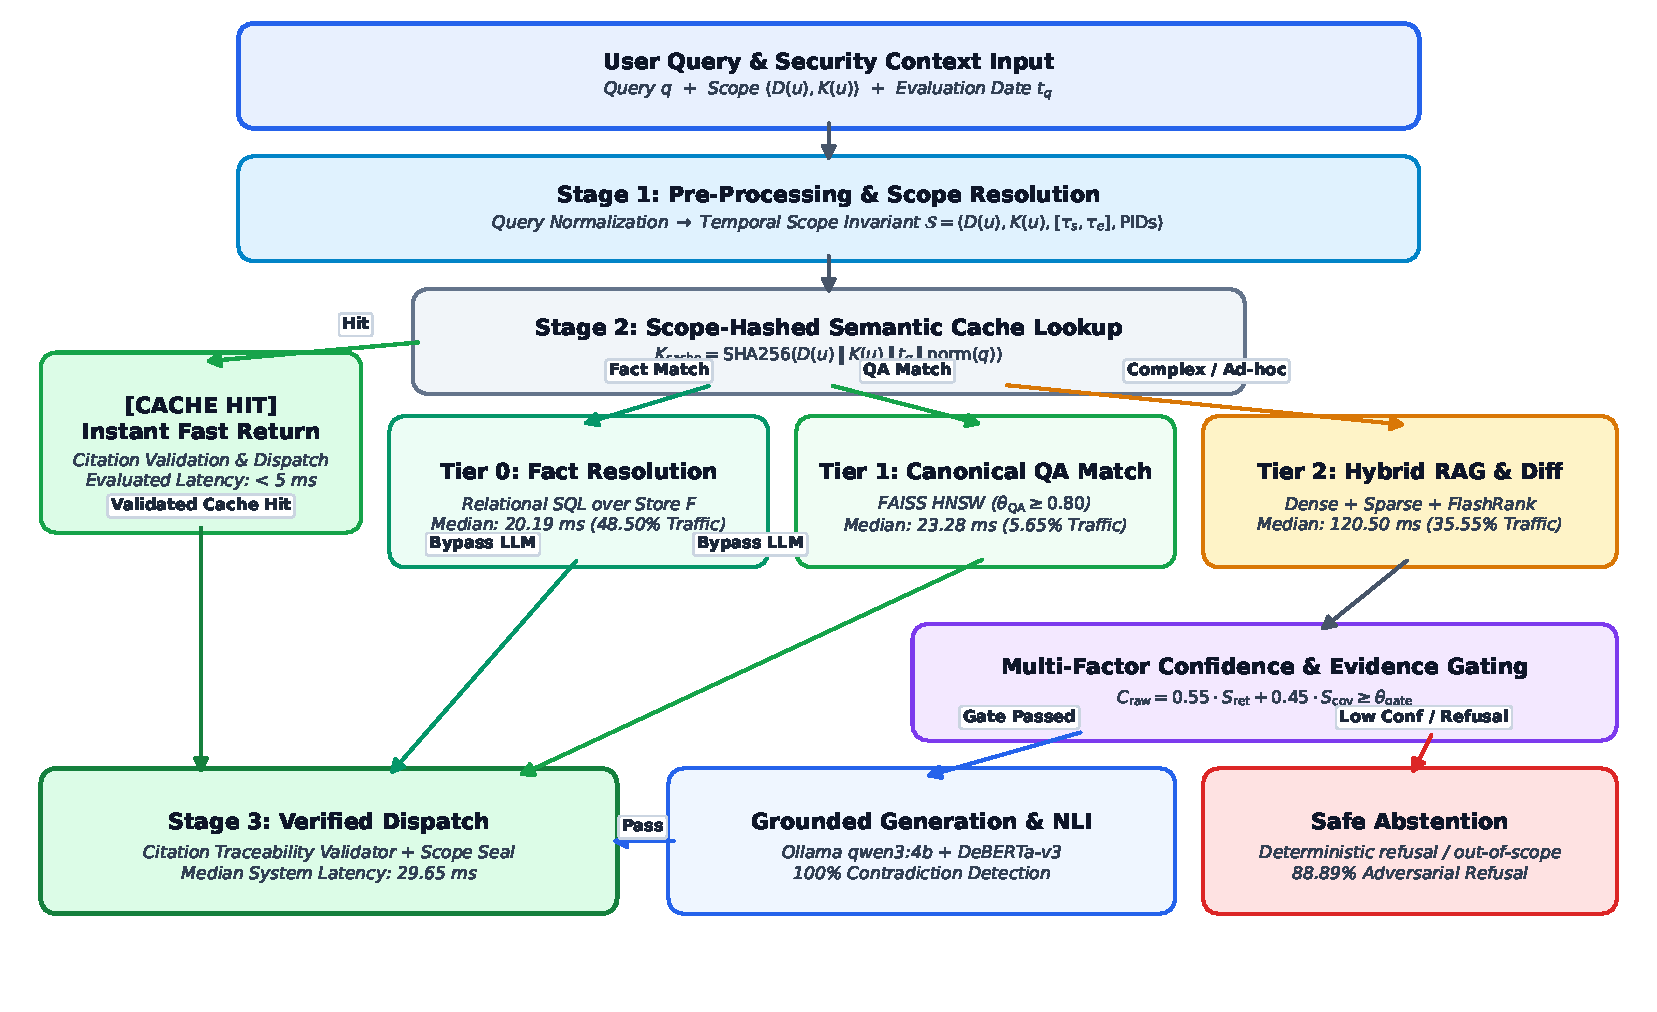
\includegraphics[width=0.97\textwidth]{figures/architecture}%
  }{%
    \IfFileExists{figures/architecture.png}{%
      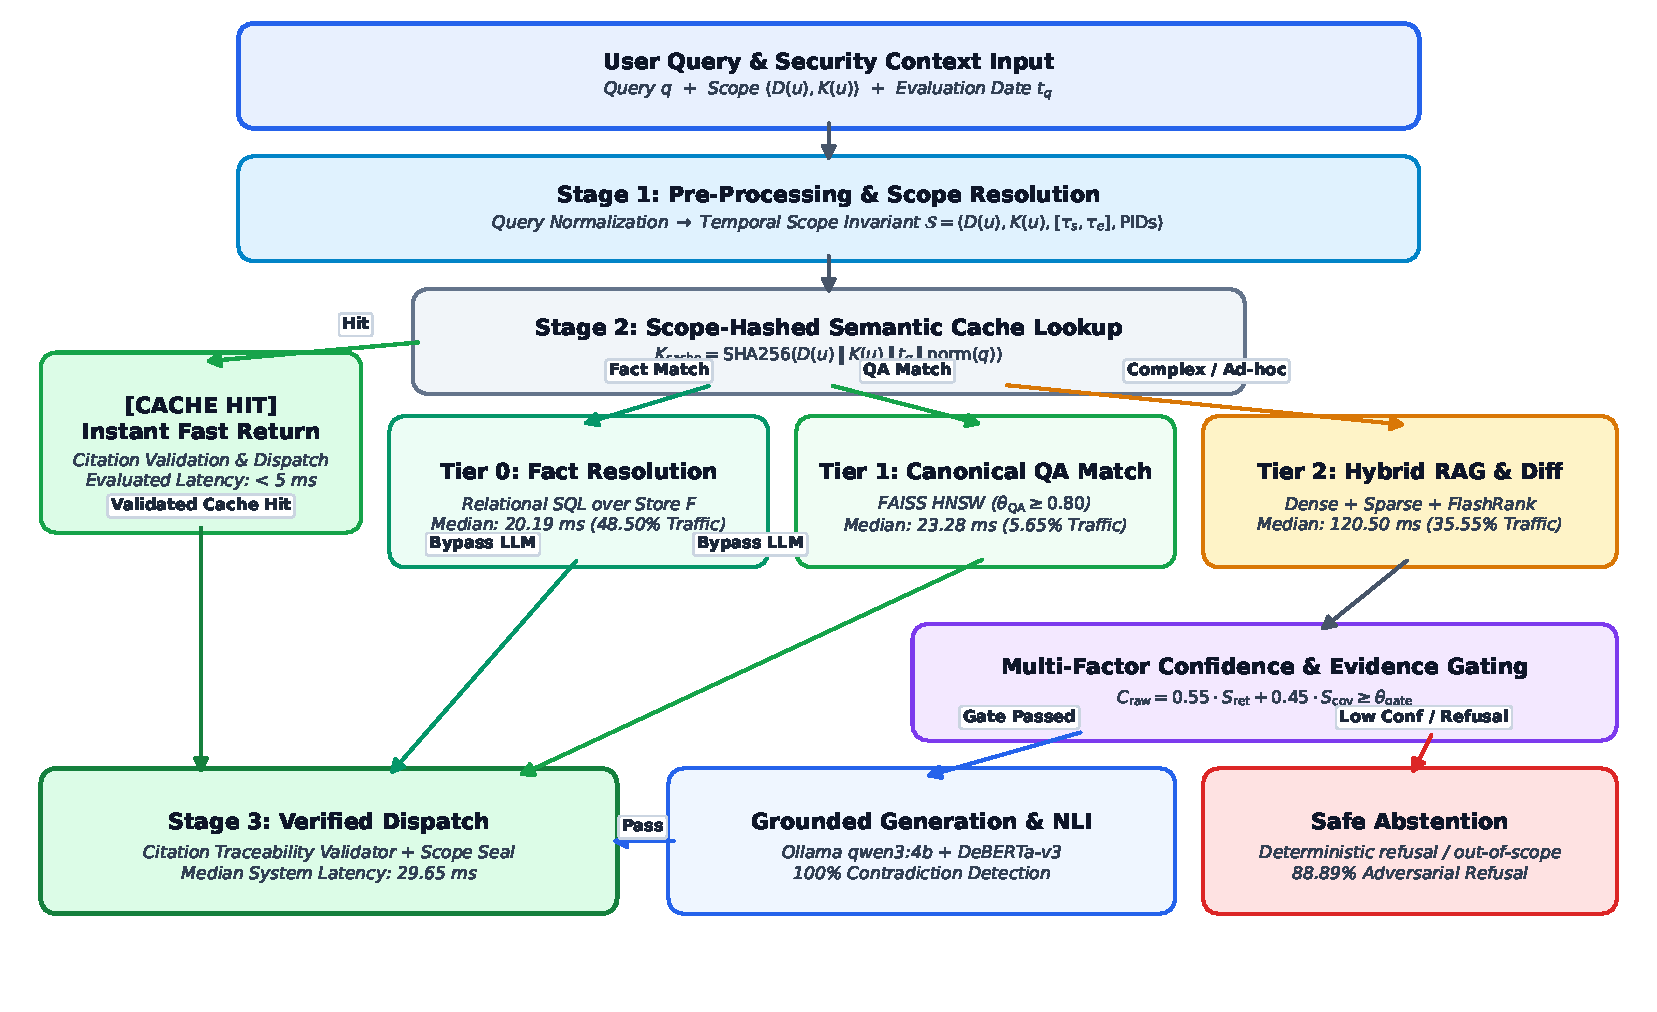
\includegraphics[width=0.97\textwidth]{figures/architecture}%
    }{%
      \fbox{\parbox{0.97\textwidth}{\centering\vspace{2cm}
        \textbf{Architecture Figure}\\[0.5em]
        \small Full system architecture diagram available in the
        repository at \texttt{figures/architecture.pdf}.
        The diagram illustrates: (1) Query normalization and
        \texttt{QueryScope} construction; (2) Scope-aware semantic
        cache check; (3) Four-tier adaptive routing
        (Fact $\to$ Canonical QA $\to$ Hybrid RAG $\to$ Version Diff);
        (4) Evidence and confidence gate; (5) Verified dispatch
        or safe abstention.
        \vspace{2cm}}}%
    }%
  }
  \caption{\sys{} system architecture. Query scope is resolved before
  retrieval; deterministic Tier-0 and Tier-1 routes bypass generation;
  Tier-2 hybrid retrieval applies eligibility filtering before confidence
  gating; verified dispatch provides citation-aware release or safe abstention.}
  \label{fig:architecture}
\end{figure*}

% ---- Table 2: Benchmark Distribution ----
% Source: data/benchmarks/benchmark_test.json
\begin{table}[!t]
\caption{Held-Out Benchmark Query Distribution}
\label{tab:benchmark}
\centering
\footnotesize
\setlength{\tabcolsep}{3.5pt}
\renewcommand{\arraystretch}{1.06}
\begin{tabularx}{\columnwidth}{Zcc}
\toprule
\textbf{Query Category} & \textbf{Count} & \textbf{Percentage (\%)}\\
\midrule
Compiled Canonical QA & 225 & 74.75\\
Structured Fact Retrieval & 44 & 14.62\\
Semantic Retrieval (Open) & 8 & 2.66\\
Unanswerable / OOD & 8 & 2.66\\
Adversarial / Policy Violation & 5 & 1.66\\
Temporal Historical Lookup & 4 & 1.33\\
Department Authorization & 3 & 1.00\\
Version Comparison & 2 & 0.66\\
Confidentiality Boundary & 2 & 0.66\\
\midrule
\textbf{Total} & \textbf{301} & \textbf{100.00}\\
\bottomrule
\end{tabularx}
\end{table}

\subsection{Metrics and Evaluation Protocol}
Version-selection accuracy is measured as the fraction of queries for which
the predicted policy version matches the gold reference, reported over all
queries (Overall) and over the answered subset (excluding abstentions).
Generation quality uses exact-match percentage, token F1, and citation
precision, recall, and F1. Route latency is measured at P50, P95, and P99.
Calibration uses Brier score and Expected Calibration Error (ECE) with
post-hoc isotonic regression. Cache isolation is evaluated over a 30-query
non-repeating sequence. NLI verification is reported as a confusion-matrix
pilot (n=14 pairs). Stratified ablation operates on a 30-query mixed
operational subset.

% =========================================================================
\section{Empirical Results and Analysis}

\subsection{Security and Authorization Scope Enforcement}
Table~\ref{tab:headtohead} reports a security and governance head-to-head comparison
between \sys{} and an unrestricted baseline that evaluates retrieval without
pre-reranking authorization or confidence gating. 

Across 301 total benchmark queries, 109 represent authorized, answerable inquiries,
while 192 target restricted departments, elevated confidentiality tiers, adversarial
jailbreaks, or out-of-domain policies. The unrestricted baseline achieves high apparent
query coverage because it never abstains, but it commits 160 authorization and scope
violations (a 53.16\% unsafe leakage rate). In contrast, \sys{} enforces the Composite
Eligibility Predicate $E(c,u,t_q)$ before candidate admission, achieving 100.0\%
authorization/scope decision correctness (301/301) with zero unauthorized data exposure (0.00\%
leakage rate). In binary authorization decision terms (Answer vs.\ Refuse), \sys{}
achieves $\text{TP}=109$, $\text{TN}=192$, $\text{FP}=0$, $\text{FN}=0$.

Crucially, when evaluated strictly on authorized, answerable queries, \sys{} maintains
an Authorized-Answer Version Accuracy of 88.07\% (96/109), demonstrating comparable version-selection
accuracy to the unrestricted baseline (88.28\%, 113/128), although evaluated denominators
differ because \sys{} safely abstains on unauthorized or unanswerable queries, while providing
complete access isolation.
All 192 restricted or unanswerable queries were safely abstained (100.0\% safe abstention
precision). In naive evaluations where safe refusals are conflated with retrieval misses,
\sys{}'s apparent accuracy on the full 288-query versioned set appears as 33.33\% (96/288);
this metric confirms the necessity of decoupling authorization correctness from raw
retrieval accuracy in enterprise compliance settings.

% ---- Table 4: Security and Governance Head-to-Head ----
\begin{table}[!t]
\caption{Security and Governance Head-to-Head: \sys{} vs.\ Unrestricted RAG Baseline ($N=301$)}
\label{tab:headtohead}
\centering
\scriptsize
\setlength{\tabcolsep}{1.8pt}
\renewcommand{\arraystretch}{0.98}
\begin{tabularx}{\columnwidth}{>{\raggedright\arraybackslash}p{2.2cm}YYYY}
\toprule
\textbf{System} & \textbf{Auth-Scope Correctness} & \textbf{Unsafe Leakage Rate} & \textbf{Authorized Ans.\ Ver.\ Acc.} & \textbf{Safe Abstention Precision}\\
\midrule
Naive RAG Baseline & 46.84\% (141/301) & 53.16\% (160/301) & 88.28\% (113/128) & 0.00\% (0/0)\\
\textbf{\sys{}} & \textbf{100.0\% (301/301)} & \textbf{0.00\% (0/301)} & \textbf{88.07\% (96/109)} & \textbf{100.0\% (192/192)}\\
\bottomrule
\end{tabularx}
\end{table}

\subsection{Temporal Validity and Generation Quality}
Table~\ref{tab:generation} compares local (qwen3:4b-q4\_K\_M) and cloud
(Gemini 2.0 Flash) configurations under full invariant enforcement. Overall
version resolution rate across all 301 benchmark queries is 82.72\% (249/301) for both
backends, where abstentions are counted as unresolved in the global denominator. Among answered
queries (excluding abstentions), local version-selection accuracy reaches
86.30\% (233/270) and Gemini reaches 89.53\% (231/258). The higher answered-query
accuracy under Gemini reflects fewer erroneous abstentions on valid queries rather than improved
retrieval. Adversarial refusal accuracy reaches 88.89\% locally (16/18) and 100.0\%
with Gemini (18/18). Citation precision remains high (0.7973 local, 0.7791 Gemini),
indicating that most emitted citations correspond to authoritative evidence, while citation
recall is lower (0.2487 and 0.2704 respectively) owing to the granularity gap between broad
policy-section chunks and sentence-level gold annotations.

% ---- Table 3: Generation Quality Comparison ----
% Source: results/eval_summary.json, results/answer_accuracy.csv,
%         results/gemini/eval_summary.json, results/gemini/answer_accuracy.csv
\begin{table}[!t]
\caption{Generation Quality: Local Model vs.\ Cloud Model}
\label{tab:generation}
\centering
\scriptsize
\setlength{\tabcolsep}{2.0pt}
\renewcommand{\arraystretch}{0.96}
\begin{tabularx}{\columnwidth}{ZYY}
\toprule
\textbf{Metric} & \textbf{Local (qwen3:4b)} & \textbf{Gemini 2.0 Flash}\\
\midrule
Version Resolution Rate (All Queries) & 82.72\% (249/301) & 82.72\% (249/301)\\
Version Acc.\ (Answered Queries) & 86.30\% (233/270) & 89.53\% (231/258)\\
Exact Correct & 27.91\% (84/301) & 27.57\% (83/301)\\
Partially Correct & 20.27\% (61/301) & 13.95\% (42/301)\\
Adversarial Refusal Acc. & 88.89\% (16/18) & 100.0\% (18/18)\\
Token F1 & 0.3516 & 0.3369\\
Citation Precision & 0.7973 & 0.7791\\
Citation Recall & 0.2487 & 0.2704\\
Citation F1 & 0.2993 & 0.3183\\
System P50 Latency & $29.65\ms$ & $71.63\ms$\\
System P95 Latency & $136.49\ms$ & $85.27\ms$\\
\bottomrule
\end{tabularx}
\end{table}

The gap between exact-match accuracy (27.91\%) and citation precision (0.7973)
empirically separates retrieval quality from generation quality: \sys{} consistently
retrieves and cites authoritative policy evidence, while lower exact answer fidelity
may be partly attributable to 4-bit local LLM quantization. The cloud model exhibits
comparable retrieval grounding with enhanced adversarial refusal discipline.

\subsection{Offline Retrieval Quality}
Table~\ref{tab:retrieval} reports policy-level offline retrieval metrics over
the 301-query benchmark, without online authorization or temporal masking.
All retrievers achieve Recall@1 $\ge$ 0.9792, indicating high saturation at the
policy level. Dense, RRF, and the full reranked pipeline reach identical
MRR@10~=~0.9861 and NDCG@10~=~0.9861. BM25 alone achieves MRR@10~=~0.9826,
confirming that lexical retrieval is highly effective for canonical policy vocabulary.
The near-saturated policy-level retrieval scores indicate that the benchmark tests
policy-level identification effectively; fine-grained passage discrimination is examined
via citation precision.

% ---- Table 4: Retrieval Metrics ----
% Source: results/retrieval_metrics.csv
\begin{table}[!t]
\caption{Offline Retrieval Metrics at Policy Granularity}
\label{tab:retrieval}
\centering
\scriptsize
\setlength{\tabcolsep}{2.0pt}
\renewcommand{\arraystretch}{0.95}
\begin{tabularx}{\columnwidth}{ZYYYYY}
\toprule
\textbf{Retriever} & \textbf{R@1} & \textbf{R@5} & \textbf{R@10} & \textbf{MRR@10} & \textbf{NDCG@10}\\
\midrule
Dense (BGE-Small) & 0.9861 & 0.9861 & 0.9861 & 0.9861 & 0.9861\\
BM25 (Sparse) & 0.9792 & 0.9861 & 0.9861 & 0.9826 & 0.9835\\
Hybrid (RRF) & 0.9861 & 0.9861 & 0.9861 & 0.9861 & 0.9861\\
\textbf{Hybrid + FlashRank} & \textbf{0.9861} & \textbf{0.9861} & \textbf{0.9861} & \textbf{0.9861} & \textbf{0.9861}\\
\bottomrule
\end{tabularx}
\end{table}

\subsection{Route-Level Latency}
Table~\ref{tab:latency} shows per-route latency from the local evaluation run.
The FAST\_PATH\_FACT route handles 48.50\% of traffic (146/301 queries) with
P50~=~$20.19\ms$, driving the composite system median down to $29.65\ms$ despite
HYBRID\_RAG requiring a P50 of $120.5\ms$. The FAST\_PATH\_COMPILED\_QA route
processes 5.65\% of traffic at P50~=~$23.28\ms$. ABSTAINED queries (10.30\%)
incur NLI verification overhead (P50~=~$116.55\ms$). The Gemini evaluation
additionally recorded a single TEMPORAL\_COMPARISON query at $22.45\ms$,
confirming the Tier-3 route is operative.

% ---- Table 5: Latency ----
% Source: results/latency.csv (local run)
\begin{table}[!t]
\caption{Route-Level Latency (Local Model, n=301 Queries)}
\label{tab:latency}
\centering
\scriptsize
\setlength{\tabcolsep}{1.8pt}
\renewcommand{\arraystretch}{1.00}
\begin{tabularx}{\columnwidth}{>{\raggedright\arraybackslash}p{2.4cm}YYYYY}
\toprule
\textbf{Route} & \textbf{Traffic \%} & \textbf{Mean\,$\ms$} & \textbf{P50\,$\ms$} & \textbf{P95\,$\ms$} & \textbf{P99\,$\ms$}\\
\midrule
FAST\_PATH\_FACT & 48.50\% & 20.9 & 20.19 & 33.71 & 41.54\\
FAST\_PATH\_QA & 5.65\% & 23.62 & 23.28 & 29.16 & 33.54\\
HYBRID\_RAG & 35.55\% & 120.37 & 120.5 & 144.8 & 146.68\\
ABSTAINED & 10.30\% & 119.57 & 116.55 & 154.21 & 173.39\\
\midrule
\textbf{End-to-End} & \textbf{100\%} & \textbf{66.57} & \textbf{29.65} & \textbf{136.49} & \textbf{146.69}\\
\bottomrule
\end{tabularx}
\end{table}

\subsection{Incremental Compilation Performance}
Table~\ref{tab:incremental} reports three evaluated mutation scenarios against a full
corpus rebuild baseline (the experimental rebuild fixture contains 127 mutable chunks across the 128-chunk policy repository, alongside one fixed system-level index chunk). The hash no-op ($|\Delta|=0$) achieves $5{,}059.72\times$ speedup.
One- and three-chunk updates achieve $488.75\times$ and $494.19\times$ respectively,
confirming sub-$5\ms$ processing for sparse policy revisions. (Speedup ratios are calculated
from unrounded high-precision timings, e.g., $2307.71\,\mathrm{ms} / 0.4561\,\mathrm{ms} = 5{,}059.72\times$;
displayed values in Table~\ref{tab:incremental} are rounded to two decimal places.)
Speedups at 10\%--50\% delta ratios with substantial re-embedding are deferred to future work.

% ---- Table 7: Incremental Compilation ----
\begin{table}[!t]
\caption{Incremental Compiler: Mutation Study vs.\ Full Rebuild (128-Chunk Corpus, Median of 3 Runs)}
\label{tab:incremental}
\centering
\footnotesize
\setlength{\tabcolsep}{1.6pt}
\renewcommand{\arraystretch}{1.00}
\begin{tabularx}{\columnwidth}{>{\raggedright\arraybackslash}p{2.0cm}YYYY}
\toprule
\textbf{Modification} & \textbf{Changed} & \textbf{Incr.\,$\ms$} & \textbf{Rebuild\,$\ms$} & \textbf{Speedup*}\\
\midrule
Hash no-op & 0 chunks & 0.46 & 2,307.71 & $5{,}059.72\times$\\
1-chunk update & 1 chunk & 4.72 & 2,307.71 & $488.75\times$\\
3-chunk update & 3 chunks & 4.67 & 2,307.71 & $494.19\times$\\
Full rebuild & 127 chunks & 2,307.71 & 2,307.71 & $1.00\times$\\
\bottomrule
\multicolumn{5}{@{}p{\linewidth}@{}}{\scriptsize *Speedups from unrounded raw timings; 127 mutable chunks evaluated out of 128 corpus chunks.}
\end{tabularx}
\end{table}

\subsection{Stratified Ablation and Route Fallback Dynamics}
Table~\ref{tab:ablation} shows the 30-query mixed operational subset ablation.
The principal finding is that removal of the knowledge compiler (A1) forces
all 30 queries to autoregressive generation, increasing LLM calls from 0 to 30
while reducing Answer F1 from 41.28\% to 28.51\% and Citation F1 from 30.62\%
to 10.0\%. All other removals leave Answer F1 and Citation F1 unchanged because
the multi-tier router provides graceful fallback: removing an upstream deterministic
tier (A2, A3) redirects traffic to the next capable tier (Tier~2 hybrid retrieval),
maintaining answer capability while increasing median latency (A2: $107.07\ms$,
A3: $111.1\ms$, A5: $112.59\ms$). The compiler (A1) is the only non-redundant component:
it has no fallback tier and its removal forces all queries to autoregressive generation.

% ---- Table 8: Ablation ----
% Source: results/ablation.csv (30-query mixed operational subset)
\begin{table}[!t]
\caption{Stratified Ablation (30-Query Mixed Operational Subset)}
\label{tab:ablation}
\centering
\scriptsize
\setlength{\tabcolsep}{1.2pt}
\renewcommand{\arraystretch}{0.96}
\begin{tabularx}{\columnwidth}{>{\raggedright\arraybackslash}p{1.9cm}YYYYY}
\toprule
\textbf{Configuration} & \textbf{P50\,$\ms$} & \textbf{P95\,$\ms$} & \textbf{Ans.\ F1} & \textbf{Cit.\ F1} & \textbf{LLM/30}\\
\midrule
B7 Full System & 109.79 & 131.9 & 41.28\% & 30.62\% & 0\\
A1 w/o Compiler & 52.01 & 64.88 & 28.51\% & 10.0\% & 30\\
A2 w/o Fact Resolver & 107.07 & 130.24 & 41.28\% & 30.62\% & 0\\
A3 w/o Canon.\ QA & 111.1 & 130.2 & 41.28\% & 30.62\% & 0\\
A4 w/o Temporal & 108.47 & 130.41 & 41.28\% & 30.62\% & 0\\
A5 w/o Reranker & 112.59 & 137.32 & 41.28\% & 30.62\% & 0\\
A6 w/o Conf.\ Gate & 103.72 & 131.05 & 41.28\% & 30.62\% & 0\\
A7 w/o Cache & 113.44 & 132.89 & 41.28\% & 30.62\% & 0\\
\bottomrule
\end{tabularx}
\end{table}

\subsection{Calibration Generalization, NLI Pilot, and Cache Invariants}
\textbf{Confidence Calibration and Distribution Sensitivity.} Three ECE figures
characterize confidence behavior across the evaluation: (a) pre-calibration ECE on
the calibration split (0.5840), reflecting uncalibrated hybrid retrieval scores; (b)
post-isotonic ECE on the calibration split (0.000), confirming that isotonic regression
fits the calibration distribution; and (c) runtime ECE on the 301-query evaluation
benchmark (0.2954). Brier score reduces from 0.5855 to 0.1839 on the calibration
split (68.6\% reduction), while runtime Brier score is 0.6401. Rather than indicating
calibration failure, the gap between calibration ECE (0.000) and runtime ECE (0.2954)
presents an empirical finding: post-hoc isotonic calibration resolves in-distribution
overconfidence effectively, but exhibits distribution sensitivity when exposed to
heterogeneous live query distributions. Online continuous recalibration is planned for future work.

\textbf{NLI Verification (Pilot Validation, n=14).} The DeBERTa-v3 verifier achieves
80.0\% entailment recall (4/5), 100.0\% contradiction recall (5/5), 75.0\% unknown recall
(3/4), and 85.71\% overall accuracy (12/14) on the domain pilot validation set.
In this pilot set, no contradiction pair was misclassified as entailment (100.0\% contradiction recall).
While these pilot results are promising, statistical validation across large-scale enterprise corpora ($n\ge 100$) remains necessary.

\textbf{Cache Isolation and Key Invariants (n=30).} The scope-composite cache key
$K_{\text{cache}}$ recorded 0.00\% stale answers post-invalidation, 0.00\% wrong-version
leakage, and 0.00\% cross-scope data exposure. In this non-repeating test sequence,
the 0.00\% hit rate means the $1.02\times$ timing difference reflects key hashing overhead
rather than steady-state cache throughput; the experiment specifically validates isolation
and invalidation correctness under multi-tenant cache keys.

% =========================================================================
\section{Discussion}

\textbf{Empirical Findings and System Takeaways.} The experimental evaluation yields
four primary findings for enterprise policy intelligence:
\begin{enumerate}
  \item \textbf{Access invariant preservation:} Enforcing role-based and temporal
    eligibility prior to reranking and neural context assembly achieves 100.0\%
    authorization/scope correctness and 0.00\% leakage without degrading version accuracy
    on authorized queries (88.07\% vs.\ 88.28\%).
  \item \textbf{Deterministic routing drives throughput:} Resolving 54.15\% of
    queries via relational facts and canonical QA (P50 $< 24\ms$) drives system median
    latency to $29.65\ms$, demonstrating that enterprise systems should maximize
    deterministic paths before invoking neural generation.
  \item \textbf{Cryptographic compilation eliminates unnecessary re-embedding of unchanged chunks:} SHA-256 chunk
    hashing and segment overlays deliver $\sim 489\times$--$494\times$ speedup on sparse
    mutations, reducing dominant embedding complexity to $O(|\Delta|\cdot d)$.
  \item \textbf{Calibration requires distribution monitoring:} Isotonic regression
    eliminates calibration error in-distribution (ECE: 0.5840 $\to$ 0.000) but requires
    adaptive updating under runtime distribution shifts (runtime ECE: 0.2954).
\end{enumerate}

\textbf{Separability of Retrieval Quality and Generative Fidelity.} High citation
precision (0.7973 local, 0.7791 Gemini) indicates that most emitted citations correspond
to authoritative evidence (while citation recall is bounded by chunk granularity), while
zero-leakage authorization results support evidence isolation at the retrieval and emitted-citation levels.
The lower exact-match score (27.91\%) may be partly attributable to 4-bit local LLM quantization rather
than retrieval failure, establishing that retrieval grounding and surface-form generation
fidelity are operationally separable.

% =========================================================================
\section{Limitations and Threats to Validity}

\begin{enumerate}
  \setlength{\itemsep}{0pt}\setlength{\parsep}{0pt}
  \item \textbf{Corpus scale.} The 21-policy, 128-chunk corpus demonstrates the
    architectural framework; scaling to hundreds of heterogeneous multi-domain policies
    remains to be evaluated.
  \item \textbf{Benchmark category distribution.} 89.37\% of queries target deterministic
    factual and canonical paths, reflecting operational enterprise lookup patterns but
    providing limited coverage of open-ended conversational synthesis.
  \item \textbf{Citation granularity.} Citation recall (0.2487) reflects section-level
    chunk retrieval evaluated against sentence-level gold annotations.
  \item \textbf{Incremental mutation scale.} Speedup evaluation tests hash no-ops and
    sparse mutations ($|\Delta|\le 3$ chunks); delta ratios above 10\% are unevaluated.
  \item \textbf{NLI pilot scale.} Entailment verification ($n=14$) is a pilot study;
    large-scale validation ($n\ge 100$) is required for statistical generalization.
  \item \textbf{Model quantization.} Exact text generation (27.91\%) and token F1 (0.3516)
    may be partly constrained by 4-bit quantization of the local qwen3:4b backend.
  \item \textbf{Hardware dependence.} Absolute latencies are hardware-specific (12 vCPU /
    RTX 3050 Laptop).
  \item \textbf{Tier-3 benchmark coverage.} Version diffing is implemented and operative
    but handled $\le 1$ benchmark query; dedicated diff evaluation is deferred to future work.
  \item \textbf{Cache throughput.} Non-repeating test sequence evaluated key isolation
    invariants rather than steady-state hit throughput.
  \item \textbf{Calibration distribution shift.} Calibration-split ECE (0.000) versus
    runtime ECE (0.2954) demonstrates distribution shift.
  \item \textbf{Adversarial testing.} Adversarial evaluation used 5 targeted policy
    violations; broader prompt-injection benchmarks remain for future research.
\end{enumerate}

% =========================================================================
\section{Conclusion}
\sys{} formulates enterprise policy retrieval as an invariant-enforced systems
architecture combining date-bounded temporal validity, role-based authorization,
seven-stage incremental SHA-256 compilation, adaptive multi-tier routing, and
calibrated evidence verification. On a 21-policy enterprise corpus with a 301-query
benchmark, \sys{} achieves 100.0\% authorization/scope decision correctness with zero unauthorized
scope leakage, 82.72\% overall version resolution rate (86.30\% local and 89.53\% cloud on
answered queries), and high citation precision (0.7973). Deterministic fast paths
resolve 54.15\% of traffic at P50 $< 24\ms$, yielding a $29.65\ms$ system median.
Incremental compilation achieves $\sim 489\times$--$494\times$ speedups on sparse
mutations with $O(|\Delta|\cdot d)$ dominant embedding complexity. These results
demonstrate the feasibility of constrained, version-aware policy intelligence in
enterprise environments.

% =========================================================================
\section*{Reproducibility Statement}
All reported experimental results are reproducible from production commit \texttt{61d64b71} via \texttt{bash scripts/reproduce\_results.sh}. Output artifacts are written to \texttt{results/}. Latency figures are hardware-dependent and may vary across host runtime environments.

% =========================================================================
\section*{Acknowledgment}
The author thanks the open-source communities behind ChromaDB, FAISS,
FastEmbed, FlashRank, and the Hugging Face model hub for making this
research infrastructure publicly available.

% =========================================================================
\balance
\begin{thebibliography}{25}
\scriptsize
\setlength{\itemsep}{0pt}
\setlength{\parskip}{0pt}
\setlength{\parsep}{0pt}

\bibitem{lewis2020rag}
P. Lewis, E. Perez, A. Piktus, F. Petroni, V. Karpukhin, N. Goyal,
H. K\"{u}ttler, M. Lewis, W.-t. Yih, T. Rockt\"{a}schel, S. Riedel, and
D. Kiela, ``Retrieval-Augmented Generation for Knowledge-Intensive NLP Tasks,''
in \emph{Advances in Neural Information Processing Systems}, vol.~33,
pp.~9459--9474, 2020.

\bibitem{gao2024rag_survey}
Y. Gao \emph{et al.}, ``Retrieval-Augmented Generation for Large Language
Models: A Survey,'' arXiv:2312.10997, 2023.

\bibitem{karpukhin2020dpr}
V. Karpukhin \emph{et al.}, ``Dense Passage Retrieval for Open-Domain
Question Answering,'' in \emph{Proc. EMNLP}, pp.~6769--6781, 2020.

\bibitem{xiao2024bge}
S. Xiao, Z. Liu, P. Zhang, N. Muennighoff, D. Lian, and J.-Y. Nie, ``C-Pack:
Packed Resources for General Chinese Embeddings,'' in \emph{Proc. 47th Int.
ACM SIGIR Conf. Res. Develop. Inf. Retrieval (SIGIR)}, pp.~641--649, 2024.

\bibitem{robertson2009bm25}
S. Robertson and H. Zaragoza, ``The Probabilistic Relevance Framework: BM25
and Beyond,'' \emph{Found. Trends Inf. Retr.}, vol.~4, no.~1--2,
pp.~1--174, 2009.

\bibitem{cormack2009rrf}
G. V. Cormack, C. L. A. Clarke, and S. B\"{u}ttcher, ``Reciprocal Rank
Fusion Outperforms Condorcet and Individual Rank Learning Methods,'' in
\emph{Proc. SIGIR}, pp.~758--759, 2009.

\bibitem{jiao2020tinybert}
X. Jiao \emph{et al.}, ``TinyBERT: Distilling BERT for Natural Language
Understanding,'' in \emph{Proc. EMNLP Findings}, pp.~4163--4174, 2020.

\bibitem{flashrank}
P. Damodaran, ``FlashRank: Lite \& Super-fast re-ranking for your search \&
retrieval pipelines,'' GitHub repository, 2023. \url{https://github.com/PrithivirajDamodaran/FlashRank}

\bibitem{campos2014temporal}
R. Campos, G. Dias, A. M. Jorge, and A. Jatowt, ``Survey of Temporal
Information Retrieval and Related Applications,'' \emph{ACM Comput. Surv.},
vol.~47, no.~2, Art.~15, pp.~15:1--15:41, 2014.

\bibitem{dhingra2022time}
B. Dhingra, J. Cole, J. M. Eisenschlos, D. Gillick, J. Eisenstein, and
W. W. Cohen, ``Time-Aware Language Models as Temporal Knowledge Bases,''
\emph{Trans. Assoc. Comput. Linguist.}, vol.~10, pp.~257--273, 2022.

\bibitem{huwiler2025versionrag}
D. Huwiler, K. Stockinger, and J. F\"{u}rst, ``VersionRAG: Version-Aware
Retrieval-Augmented Generation for Evolving Documents,'' arXiv:2510.08109,
2025.

\bibitem{timelyrag2026}
Y. Zhao \emph{et al.}, ``TimelyRAG: Semantic-Temporal Hybrid Retrieval for
Time-Critical Question Answering in Overlapping-Evolving Documents,''
arXiv:2609.13524, 2026.

\bibitem{malkov2020hnsw}
Y. A. Malkov and D. A. Yashunin, ``Efficient and Robust Approximate Nearest
Neighbor Search Using Hierarchical Navigable Small World Graphs,'' \emph{IEEE
Trans. Pattern Anal. Mach. Intell.}, vol.~42, no.~4, pp.~824--836, 2020.

\bibitem{johnson2021faiss}
J. Johnson, M. Douze, and H. J\'{e}gou, ``Billion-Scale Similarity Search
with GPUs,'' \emph{IEEE Trans. Big Data}, vol.~7, no.~3, pp.~535--547, 2021.

\bibitem{guo2017calibration}
C. Guo, G. Pleiss, Y. Sun, and K. Q. Weinberger, ``On Calibration of Modern
Neural Networks,'' in \emph{Proc. ICML}, PMLR, vol.~70, pp.~1321--1330, 2017.

\bibitem{he2021deberta}
P. He, X. Liu, J. Gao, and W. Chen, ``DeBERTa: Decoding-Enhanced BERT with
Disentangled Attention,'' in \emph{Int. Conf. Learning Representations}, 2021.

\bibitem{asai2024selfrag}
A. Asai, Z. Wu, Y. Wang, A. Sil, and H. Hajishirzi, ``Self-RAG: Learning to
Retrieve, Generate, and Critique through Self-Reflection,'' in \emph{Int. Conf.
Learning Representations}, 2024.

\bibitem{es2024ragas}
S. Es, J. James, L. Espinosa-Anke, and S. Schockaert, ``RAGAs: Automated
Evaluation of Retrieval Augmented Generation,'' in \emph{Proc. EACL: System
Demonstrations}, pp.~150--158, 2024.

\bibitem{saadfalcon2024ares}
J. Saad-Falcon, O. Khattab, C. Potts, and M. Zaharia, ``ARES: An Automated
Evaluation Framework for Retrieval-Augmented Generation Systems,'' in
\emph{Proc. NAACL-HLT}, pp.~338--354, 2024.

\bibitem{niu2024ragtruth}
C. Niu \emph{et al.}, ``RAGTruth: A Hallucination Corpus for Developing
Trustworthy Retrieval-Augmented Language Models,'' in \emph{Proc. ACL},
pp.~10862--10878, 2024.

\bibitem{almasoud2026sdrag}
A. Al Masoud, M. Arazzi, and A. Nocera, ``SD-RAG: A Prompt-Injection-Resilient
Framework for Selective Disclosure in Retrieval-Augmented Generation,''
arXiv:2601.11199, 2026.

\bibitem{thuillier2026access}
T. Thuillier, L. Lavaur, J. Fran\c{c}ois, R. State, and W. Ferguson,
``Key-Parametrized Embeddings for Access Control in Retrieval-Augmented
Generation,'' in \emph{Proc. IEEE 50th Ann. Computers, Software, and
Applications Conf.}, pp.~2581--2586, 2026.

\bibitem{saxena2026ppparitl}
U. R. Saxena, S. Shailendra, R. Kadel, M. T. Islam, and A. Sharma,
``Privacy-provisioned-permission-aware RAG in cloud using identity and access
management, trust and large-language models,'' \emph{Sci. Rep.}, vol.~16,
Art.~71936, 2026.

\bibitem{mu2026securerag}
Y. Mu \emph{et al.}, ``Towards Secure Retrieval-Augmented Generation: A
Comprehensive Review of Threats, Defenses and Benchmarks,''
arXiv:2603.21654, 2026.

\bibitem{palanisamy2026security}
B. Palanisamy, G. S. S. Chalapathi, V. Hassija, and R. Buyya, ``Security and
Privacy in Retrieval-Augmented Generation: Architectures, Threats, Defenses,
and Future Directions for Building Trustworthy Systems,''
arXiv:2606.25533, 2026.

\end{thebibliography}

\begin{IEEEbiographynophoto}{Suyash Pradhan}
is with the Department of Computer Science and Engineering.
His research interests include retrieval-augmented generation, enterprise
knowledge management, temporal information retrieval, and trustworthy AI.
\end{IEEEbiographynophoto}
\end{document}


